% !TEX root =  ../report.tex

\section{Implementation}
\label{s:impl}
The source code for the OP2 Framework is hosted open source as a GitHub\cite{OP2rep} repository. Instructions for obtaining the implementation described in the following section, and for getting started with OP2, are provided be found in Appendix \ref{app:getStart}.
\subsection{Git Repository}
The feature branch for this project is named \verb|feature/jit|, and was branched from \verb|feature/lazy-execution| on 13th November 2019. The last commit on the \verb|lazy-execution| was in April 2018, and therefore lagged behind the \verb|master| branch somewhat. It was rebased onto \verb|master| before any other changes were made.
\par
In git terminology, a rebase involves making copies of a branch's commits, and "re-playing" the changes made in them to the top of another branch \cite{scm-rebase}. In this case, making copies of all commits made to \verb|feature/lazy-execution| and applying them to the latest commit of \verb|master|. The result once any merge conflicts are resolved will be a codebase with all the features of both branches available.
\begin{figure}[h!]
  \caption{Rebase vs. Merge. Diagram reproduced from \cite{scm-rebase}}
  \label{fig:git_merge}
  \makebox[\textwidth][c]{
  \resizebox{1.1\textwidth}{!}{
    \begin{tikzpicture}[node distance=3.5cm, auto]

      %
      % Initial
      %

      \tikzstyle{label} = [rblock, text width=7em, minimum height=2em, fill=green!30]

      \node [wfile] (C0) {C0};
      \node [wfile, right of=C0] (C1) {C1};
      \node [wfile, right of=C1] (C2) {C2};
      \node [jfile, above=1cm of C2] (C3) {C3};
      \node [label, above=1cm of C3] (fhead) {feature/HEAD};
      \node [label,  below=1cm of C2] (mhead) {master/HEAD};

      \node [above=2em of C0] (initial) {\LARGE Initial State};

      \path [line] (C1) -- (C0);
      \path [line] (C2) -- (C1);
      \path [line] (C3.south west) -- (C1.north east);
      \path [thinline] (fhead) -- (C3);
      \path [thinline] (mhead) -- (C2);

      %
      % Rebase
      %

      \node [wfile, below=6cm of C0] (fC0) {C0};
      \node [wfile, right of=fC0] (fC1) {C1};
      \node [wfile, right of=fC1] (fC2) {C2};
      \node [jfile, above=1cm of fC2, opacity=0.2] (fC3) {C3};
      \node [label, below=1cm of fC2] (fmhead) {master/HEAD};

      \node [above=2em of fC0] (rebase) {\LARGE Rebased Commits};

      \node [jfile, right of=fC2] (fC3prime) {C3'};
      \node [label, above=1cm of fC3prime] (ffhead) {feature/HEAD};

      \path [line] (fC1) -- (fC0);
      \path [line] (fC2) -- (fC1);
      \path [line, opacity=0.2] (fC3.south west) -- (fC1.north east);
      \path [thinline] (ffhead) -- (fC3prime);
      \path [line] (fC3prime) -- (fC2);
      \path [thinline] (fmhead) -- (fC2);

      %
      % Merge
      %

      \node [wfile, right=3cm of fC3prime] (mC0) {C0};
      \node [wfile, right of=mC0] (mC1) {C1};
      \node [wfile, right of=mC1] (mC2) {C2};
      \node [jfile, above=1cm of mC2] (mC3) {C3};
      \node [label, above=1cm of mC3] (mfhead) {feature/HEAD};

      \node [wfile, right of=mC2] (mC4) {C4};
      \node [label, below=1cm of mC4] (mmhead) {master/HEAD};

      \node [above=2em of mC0] (merge) {\LARGE Merged Commits};

      \path [line] (mC1) -- (mC0);
      \path [line] (mC2) -- (mC1);
      \path [line] (mC3.south west) -- (mC1.north east);
      \path [line] (mC4) -- (mC2);
      \path [line] (mC4.north west) -- (mC3.south east);
      \path [thinline] (mfhead) -- (mC3);
      \path [thinline] (mmhead) -- (mC4);

    \end{tikzpicture}
    }}
\end{figure}
\par
Rebasing is preferable to simply merging for integrating another branch's changes as the result is a linear branch history, rather than creating a diamond. Also, in the case of merge conflicts - where a change has been made in both branches and one needs to be selected - a rebase command will stop at the first conflicting commit and allow the conflict to be resolved \cite{rebase-doc}. Synchronising using merge would result in receiving all conflicts in one go, which can make it harder to resolve.
\par
The downside of rebasing is it can be harder to recover from an erroneous rebase, than an erroneous merge. This is due to the fact that merges are not destructive, since they do not re-write history in the same way as a rebase. This will not be an issue here however.
\par
The \verb|feature/lazy-execution| branch was created for developing a system to execute parallel loops when values are required, rather than when they are called. This functionality will be achieved using an internal library function:
\codeline{void op_enqueue_kernel(op_kernel_descriptor *desc)}{op2/c/src/core/op\_lazy.cpp [71-89]}
Currently this function executes the queued loop as soon as it is invoked, but there is ongoing work into determining when the result of the loop will be needed, and potentially compressing multiple queued actions into fewer at this time. Lazy execution will not be the focus of this project, however the process for invoking parallel loops will be utilised throughout the work done to enable Just-In-Time Compilation for CUDA, so that future efforts towards lazy execution can continue on top of the JIT compilation implementation.

\subsection{Code Generation}
\label{ss:codegen}
As described in the Specification before, the majority of the implementation is made up of a Python code generation script which can be found inthe folder: \verb|translator/c/python/jit/op2_gen_cuda_jit.py| of the OP2 repository.
\\
Its entry point function is:
\pyline{def op2_gen_cuda_jit(master, date, consts, kernels)}{translator/c/python/jit/op2\_gen\_cuda\_jit.py [102]}
This function is called from another Python script \verb|op2.py| which is in the parent directory: \verb|translator/c/python/|\\
The arguments passed to it when it is called are:\\
\begin{tabular}{>{\bfseries}l l}
  master: & The name of the Application's master file \\
  date: & The exact date and time of code generation \\
  consts: & list of constants, with their type, dimension and name \\
  kernels: & \parbox[t]{.8\textwidth}{list of kernel descriptors, where each kernel is a map containing many fields describing the kernel. The values may alter the way the code for that loop is generated.}
\end{tabular}
\\
\\
The code generator first performs a check across all kernels to see if any use the Struct of Arrays data layout \cite[p13]{manual}, or if all are using the default Array of Structs. Then, a folder \verb|cuda/| is created if it doesn't exist, and the script will iterate over each kernel, generating both the Ahead-Of-Time (AOT) kernel file, and the Just-In-Time (JIT) kernel file simultaneously. In the System Digram from Section \ref{s:spec} (Figure \ref{fig:jit_sys}) these files were referred to as "Kernels" and "Optimised Kernels" respectively. \par
The generation of the Modified Application File is handled by \verb|op2.py|, and does not need to change to meet the requirements of this project.
\clearpage For each parallel loop, the two kernel files are generated with the following naming scheme:
\begin{itemize}
\vspace{-1em}
\item{\verb|AOT: cuda/[name]_kernel.cu|}
\vspace{-1em}
\item{\verb|JIT: cuda/[name]_kernel_rec.cu|}
\end{itemize}

The AOT kernel file is generated such that it doesn't just invoke the run-time compiler, but has the ability to execute the loop without requiring JIT compilation as well. The compiler invokation is wrapped in a pre-processor conditional, so that the feature can be enabled or disabled using a compiler argument to define a flag.
\\A single master kernels file Is also generated, which is shared by all parallel loops:
\begin{itemize}
\vspace{-1em}
\item{\verb|cuda/[application]_kernels.cu|}
\end{itemize}
It will contain function definitions required by all loops, or by the master application file; as well as include statements for each of the parallel loops' AOT kernels so they are collated into a single file by the compiler.

\subsubsection{Kernel Files}
\label{ss:krnl_files}
As mentioned above, the code generator creates two kernel files for each parallel loop. The following section details each of the functions that will be generated, and Figures \ref{fig:jit_include}-\ref{fig:loop_func} show the progression of each of the kernel files for an parallel loop. There is a summary on page \pageref{impl_summary} if the detail is superfluous for your needs.
\par
It is recommended to follow this section with either the translations script, or a generated kernel file, since it is not practical to include full code listings on each page. The inclusion of Figures \ref{fig:jit_include}-\ref{fig:loop_func} is only for purposes of highlighting the relevant sections of each file, and the generated code in the figures is not intended to be a legible size.

% May need to move
\clearpage
%
\begin{wrapfigure}[21]{r}{.33\textwidth}
  \centering
  \caption{JIT includes}
  \label{fig:jit_include}
  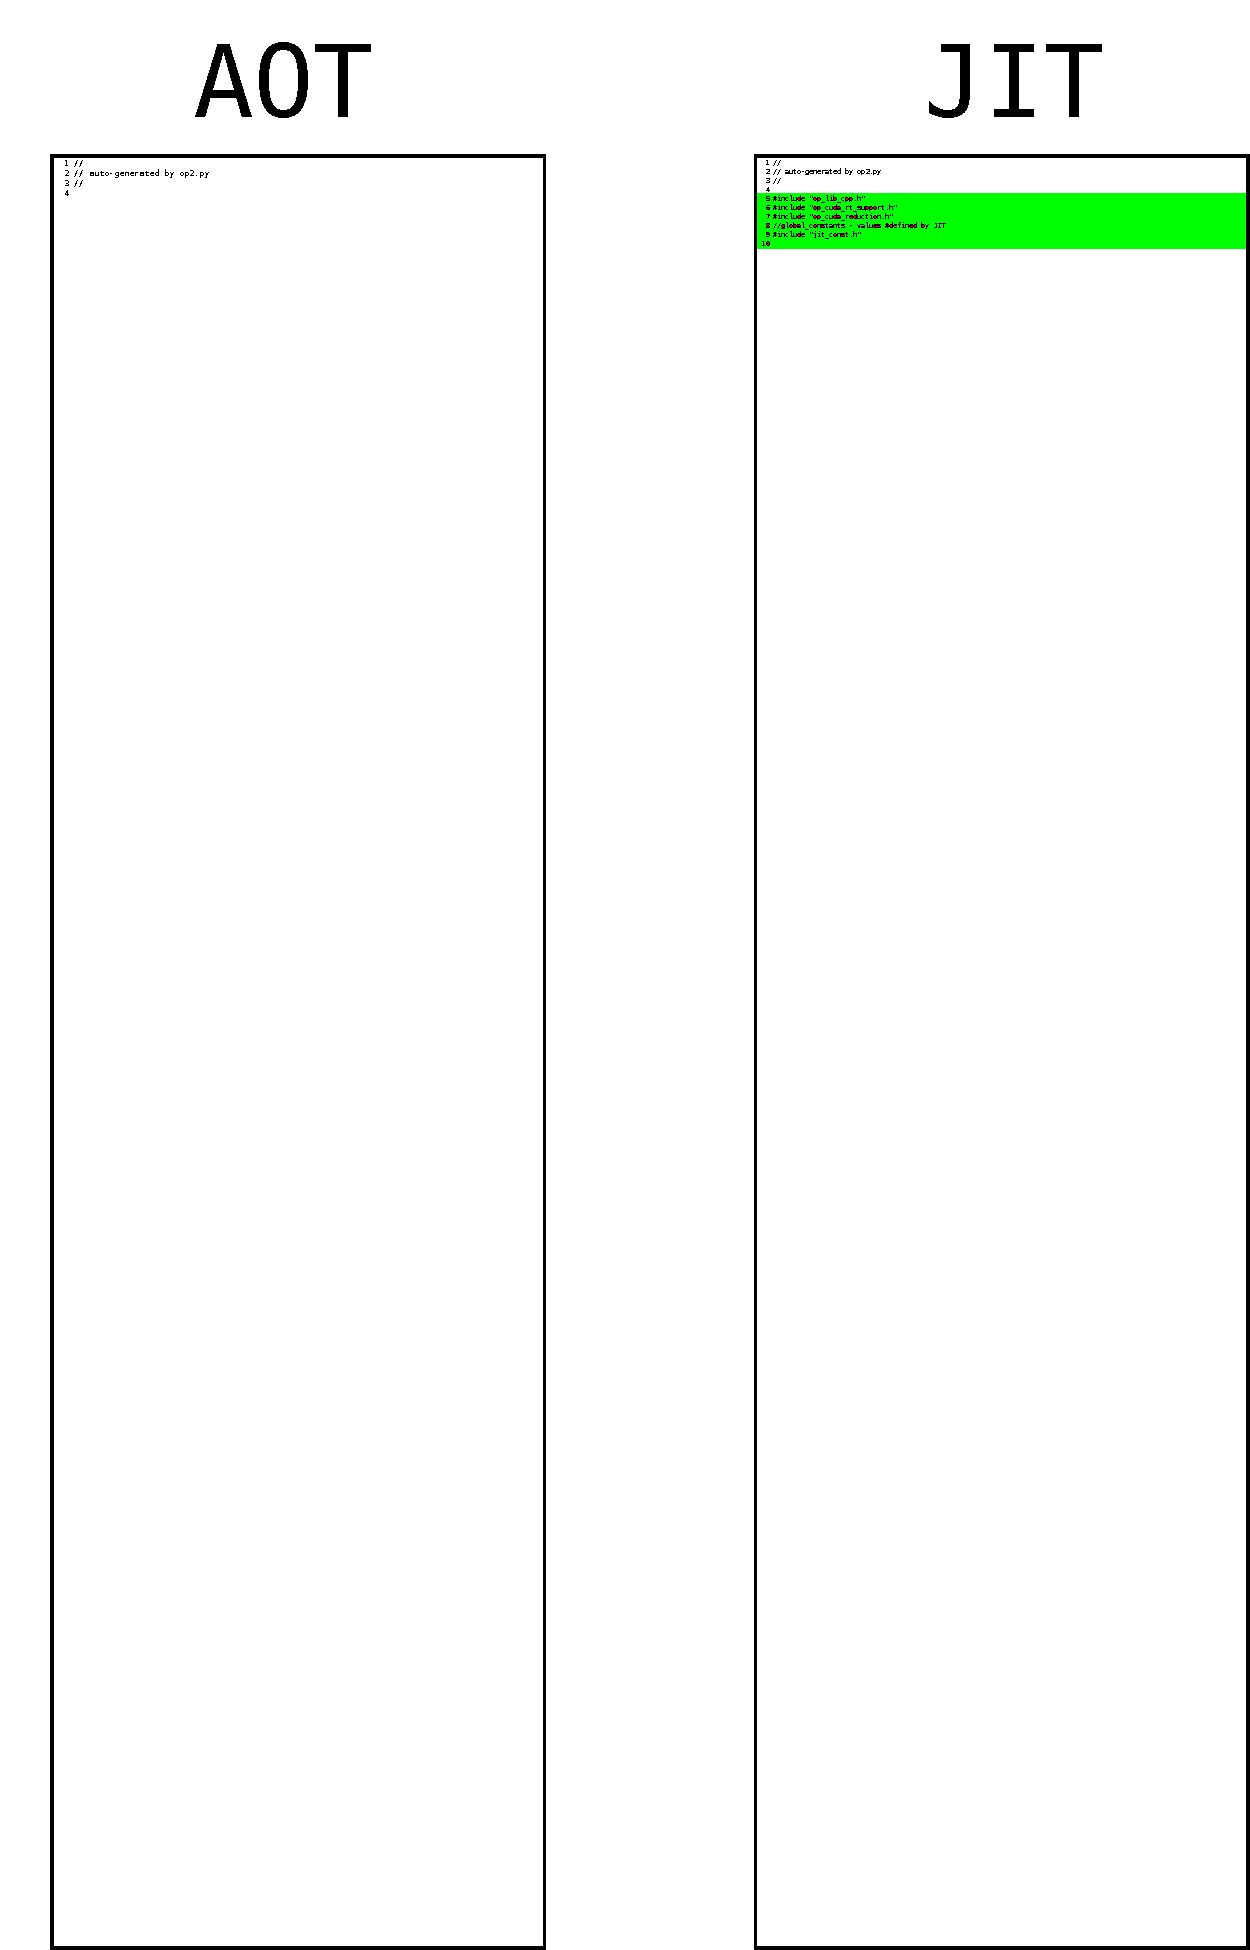
\includegraphics[width=.3\textwidth]{jit_include}
\end{wrapfigure}
\minititle{JIT includes}
The first piece of C code generated by the Python script is simply the include directives required for the JIT compiled kernel. These are needed for JIT compiled kernels since they will be processed individually by the compiler, so each requires a reference to the OP2 library files. They are not needed by the AOT kernel, as they will be included in the master kernels file, which in turn includes each of the AOT kernel files to produce a single file with all of the AOT kernels and these same \verb|#include| statements:
\begin{lstlisting}[backgroundcolor = \color{green!20}, language=C]
 #include `op_lib_cpp.h'
 #include `op_cuda_rt_support.h'
 #include `op_cuda_reduction.h'
 ...
\end{lstlisting}
The \verb|jit_const.h| file is also included, which will be generated at run-time (before the compiler is invoked) to contain a \verb|#define| for all input constants, to be handled by the pre-processor.
\begin{lstlisting}[backgroundcolor = \color{green!20}, language=C]
 ...
 //global_constants
 #include `jit_const.h'
\end{lstlisting}

\minititle{User Function}
The User Function is the kernel operation specified by the user to be carried out on each iteration of the loop, so this function will run on the device (GPU) at least once for each set item.

\begin{wrapfigure}[12]{r}{.33\textwidth}
  \centering
  \caption{User Function}
  \label{fig:usr_func}
  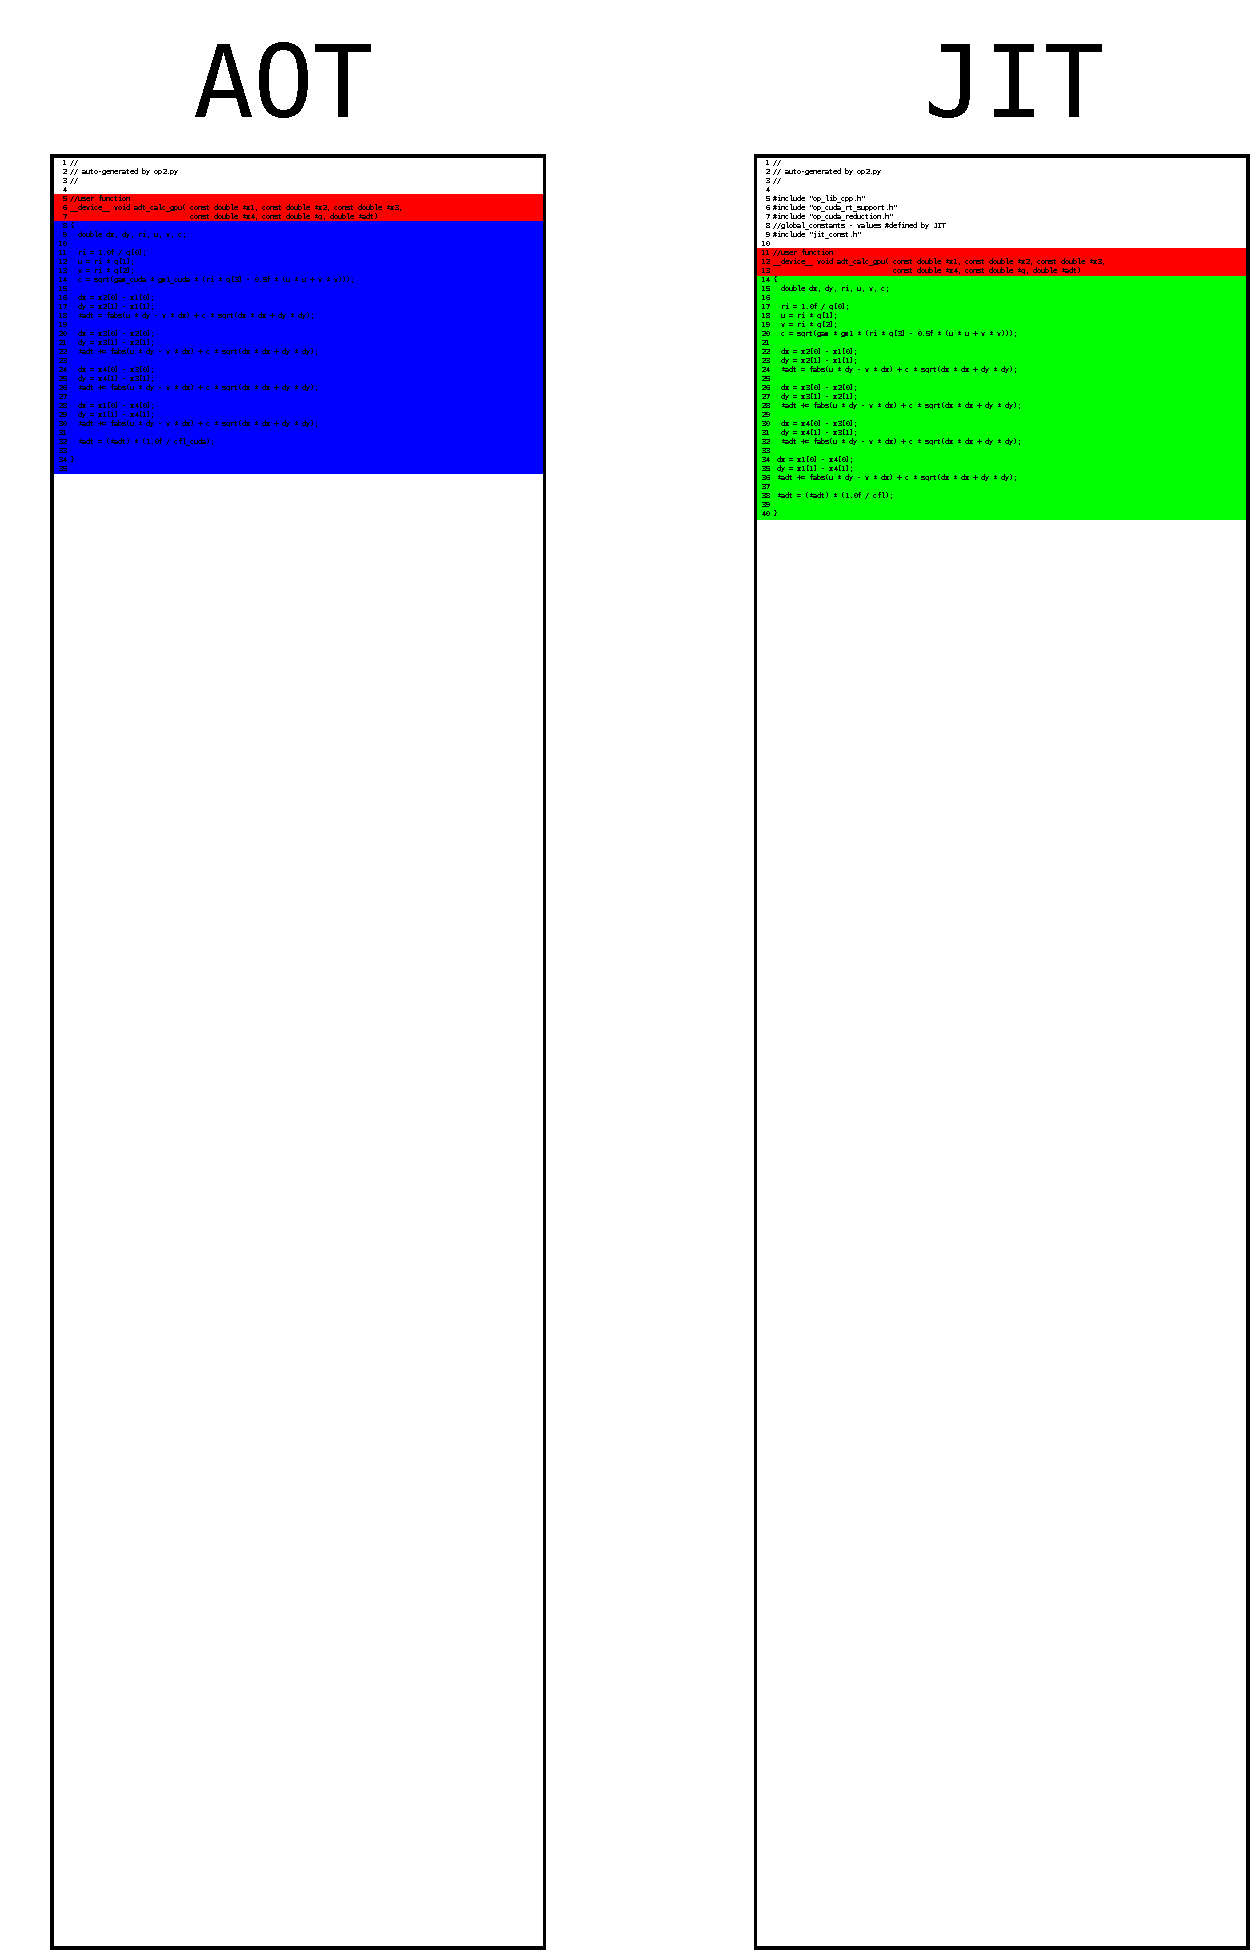
\includegraphics[width=.3\textwidth]{user_function}
\end{wrapfigure}
The User Function is given the \verb|__device__| function  descriptor, so that it will be compiled for execution on a GPU device, and can only be called from other device code - which will be the next function generated. The whole signature for the function will be:
\codeline{__device__ void [name]_gpu ( [args] )}{}
\noindent The function body will be pulled from either the application file or a header file, and is checked to ensure it has the correct number of parameters. Any include statements are replaced by the contents of the file, exactly as the pre-processor would.
\par
\tinytitle{Data Layout} If the Struct of Arrays data layout is not requested, the function body will remain largly the same as defined by the application programmer. If it is enabled however there are modifications that need to be made to support this. The code to do this is pulled from the AOT CUDA code generation script: \\\verb|translator/c/python/aot/op2_gen_cuda_simple.py|.
\par
Since the modifications involve constant values for the stride of different data structures, an attempt to streamline this process using the same constant definition optimisation was made during this project. It was unsuccessful, with a longer discussion on why later in the report.
\par
\tinytitle{Optimisations} The constant definition optimisation only needs to be applied to the user function, as it is the only one containing code written by the application developer. Wherever an input constant is referenced it needs to be modified in both the AOT and JIT kernel, but in different ways.

\tinytitle{AOT}
In the Ahead-Of-Time kernel, which will only be executed if JIT compilation is disabled, the constant will need to read from the device's memory - having been copied there when it is defined constant. The copied version will have the identifier \verb|[id]_cuda| to prevent a name collision, so all constants in the AOT kernel must be replaced with this pattern, using the following lines from the translator script:\\
\begin{lstlisting}[backgroundcolor = \color{lightgray!20}, language=Python]
for nc in range(0,len(consts)):
  varname = consts[nc]['name']
  aot_user_function = re.sub('\\b' + varname + '\\b',
                              varname + '_cuda',
                              aot_user_function)
\end{lstlisting}
\codelabel{translator/c/python/jit/op2\_gen\_cuda\_jit.py [905-907]}

\tinytitle{JIT}
The JIT kernel is a little different: contants with a dimension of 1 (i.e. they contain only 1 value) can be left the unchanged, as the value will be defined under that same identifier. There is no chance of a name collision here since the idenifier will never be allocated memory, only replaced by a literal value.
\par
Multi-Value proved more of a challenge - since values cannot be declared both \verb|__constant__| and defined as external using \verb|extern| \cite[p126]{guide}, which is how they are handled for the sequential JIT implementation.
\par
The eventual solution to this challenge was in two parts. For each index \verb|N| of the constant array, a 1 dimensional constant would be defined with the name: \verb|op_const_[id]_[N]|. All references to the constant where the index is a literal number can be replaced with the new identifier:
\begin{lstlisting}[backgroundcolor = \color{lightgray!20}, language=Python]
for nc in range(0,len(consts)):
  varname = consts[nc]['name']
  if consts[nc]['dim'] != 1:
    jit_user_function = re.sub(`\\b' + varname + `\[([0-9]+)\]',
                               `op_const_' + varname + `_\g<1>',
                                jit_user_function)}
\end{lstlisting}
\codelabel{translator/c/python/jit/op2\_gen\_cuda\_jit.py [931-934]}

If the constant is accessed using any expression other than a integer literal, this system will run into an issue, as the result of processing:
\begin{lstlisting}[frame=none,backgroundcolor=\color{white}]

int A = c_array[1+2]
\end{lstlisting}
Will be:
\begin{lstlisting}[frame=none,backgroundcolor=\color{white}]
int A = op_const_c_array_1+2
\end{lstlisting}
\noindent Which will not (in this case) result in an undefined indentifier, but the whole meaning has changed.
To resolve this, an array is defined at the top of the function with the identifier \verb|op_const_[name]|, with each index being the constant for that position. The accesses still use the expression for an index, but are modified to instead access the new array, so that the meaning is preserverd. This is only done when an expression index is found and the process becomes necessary, since allocating a new array can take time.
\begin{lstlisting}[frame=none,backgroundcolor=\color{white}]

__constant__ int op_const_c_array = { op_const_c_array_1, ...}
 ...
int A = op_const_c_array[1+2]
\end{lstlisting}
Below rest of the Python code for handling constants in the JIT compiled kernel.
\begin{lstlisting}[backgroundcolor = \color{lightgray!20}, language=Python]
for nc in range(0,len(consts)):
  ...
  jit_user_function, numFound = re.subn(`\\b' + varname + `\[',
                                      `op_const_' + varname + `[',
                                       jit_user_function)
  #At least one expression access
  if (numFound > 0):
    if CPP:
      #Line start
      codeline = `__constant__ ' + consts[nc]['type'][1:-1] +
                 ` op_const_' + varname + `[' +
                  consts[nc]['dim'] + `] = {'
      #Add each value to line
      for i in range(0,int(consts[nc][`dim'])):
          codeline += `op_const_' + varname + `_' + str(i) + `, '
      codeline = codeline[:-2] + `};'

      jit_user_function = codeline+'\n\n'+jit_user_function
\end{lstlisting}
\vspace{-1em}
\hspace*{\fill}\footnotesize{translator/c/python/jit/op2\_gen\_cuda\_jit.py [931-944]}

\begin{wrapfigure}[17]{r}{.33\textwidth}
  \vspace{-1.2cm}
  \centering
  \caption{Kernel Function}
  \label{fig:krnl_func}
  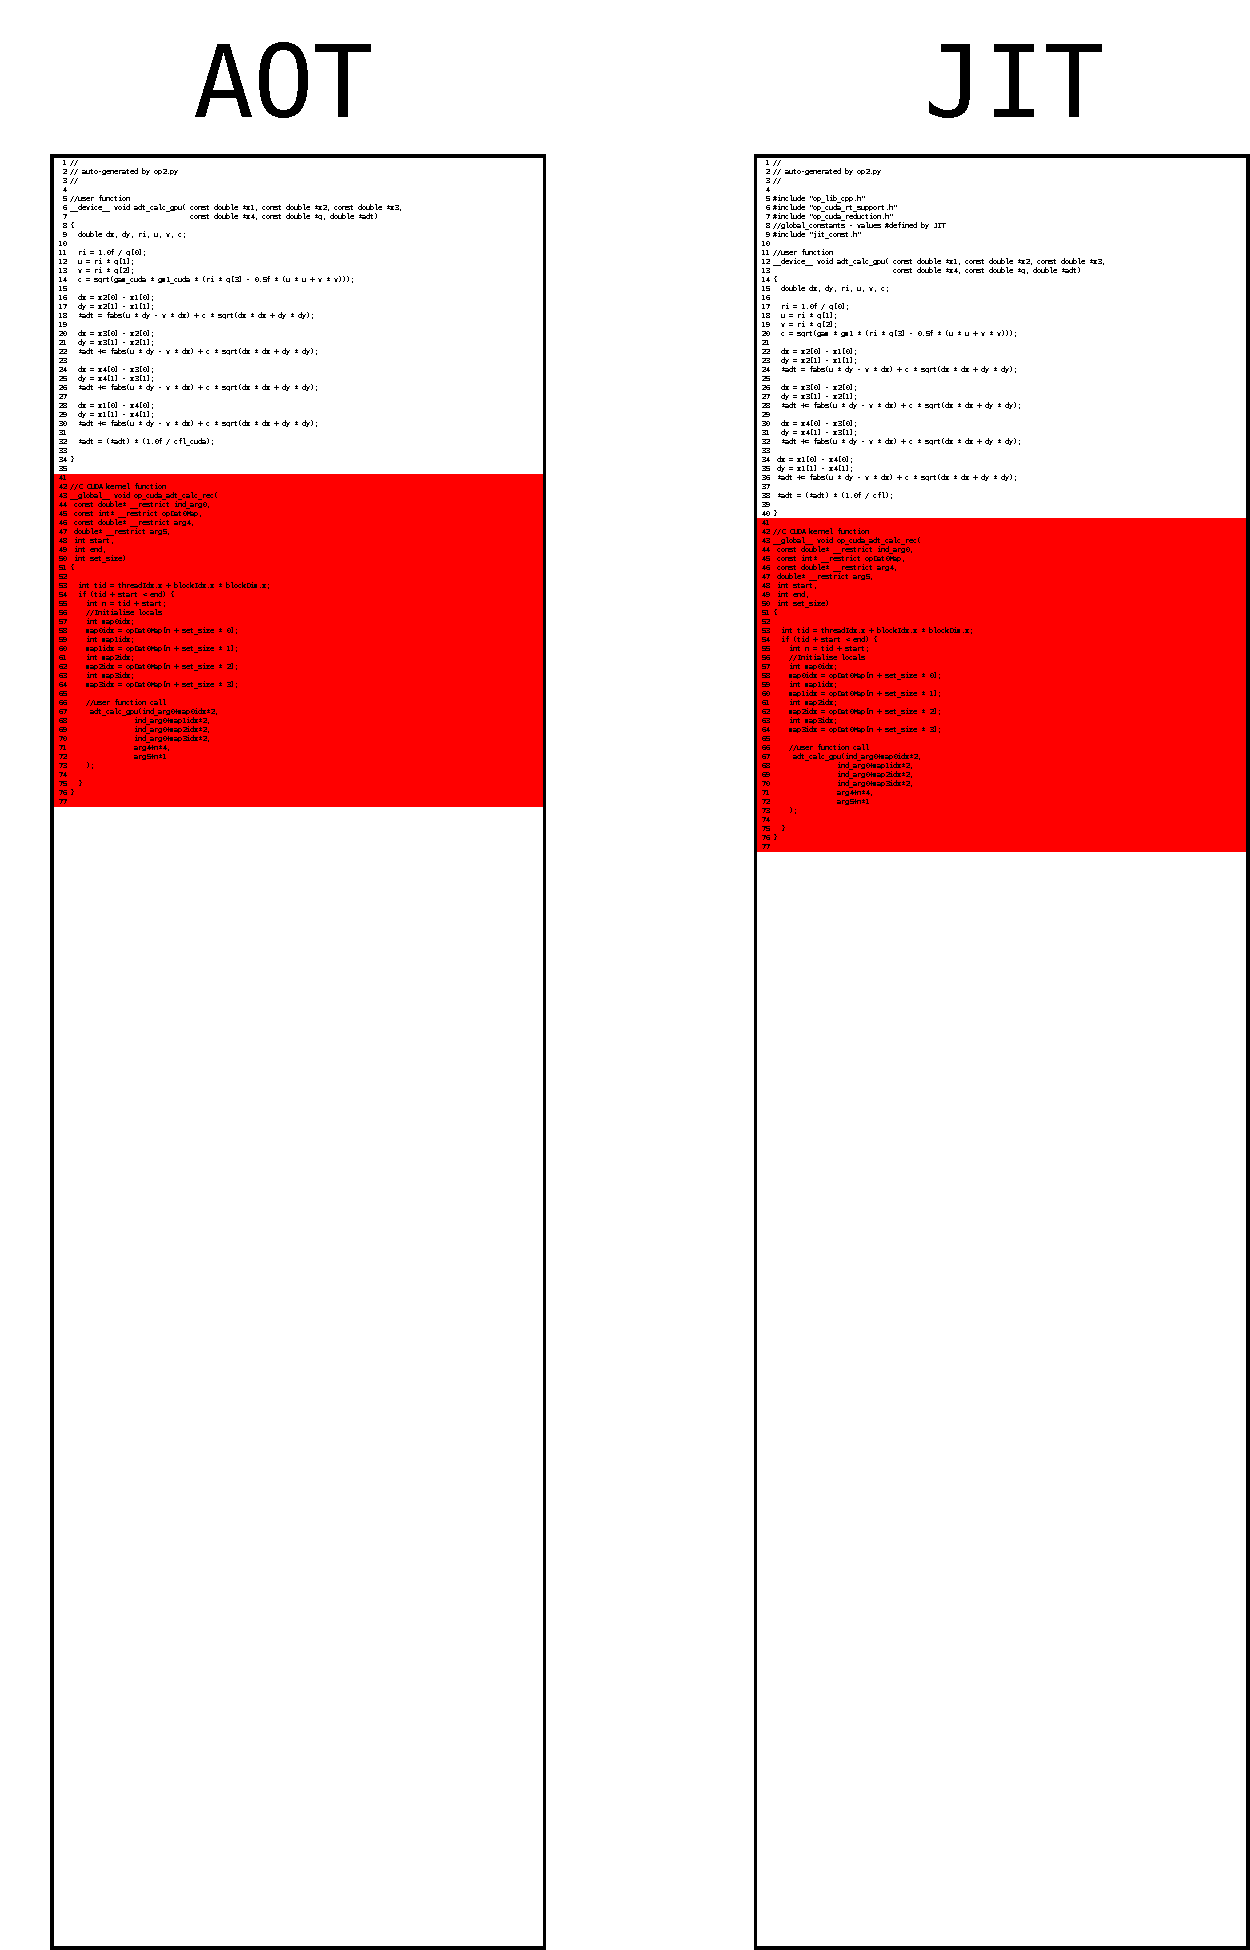
\includegraphics[width=.3\textwidth]{kernel_function}
\end{wrapfigure}
\minititle{Kernel Function}
From here onward, all code generated is based only on the kernel descriptor, and not the code that the user wrote for the body of the loop. The kernel function is the same in both files, and is executed on the GPU. It is declared \verb|__global__| so that is exectuted on the device, but can be called from host (CPU) code:
\codeline{__global__ void op_cuda_'+name+'( [args] )}{}
The function arguments depend on whether any of the arguments are optional, and whether the loop uses indirection - accessing a set using an index which is the value in another set. OP2 enforces that the operands in the set operations are referenced through at most a single level of indirection \cite[p4]{manual}.
\par
The function body also depends on whether there is indirection, as the indicies need to be retrieved from the inner map. A call is made to the user function generated above, then any reductions on arguments needs to be done. The supported reductions are: sum, maximum, and minimum\cite[p11]{manual}.

\begin{wrapfigure}[8]{r}{.33\textwidth}
  \vspace{-1.5cm}
  \centering
  \caption{Host Function}
  \label{fig:host_func}
  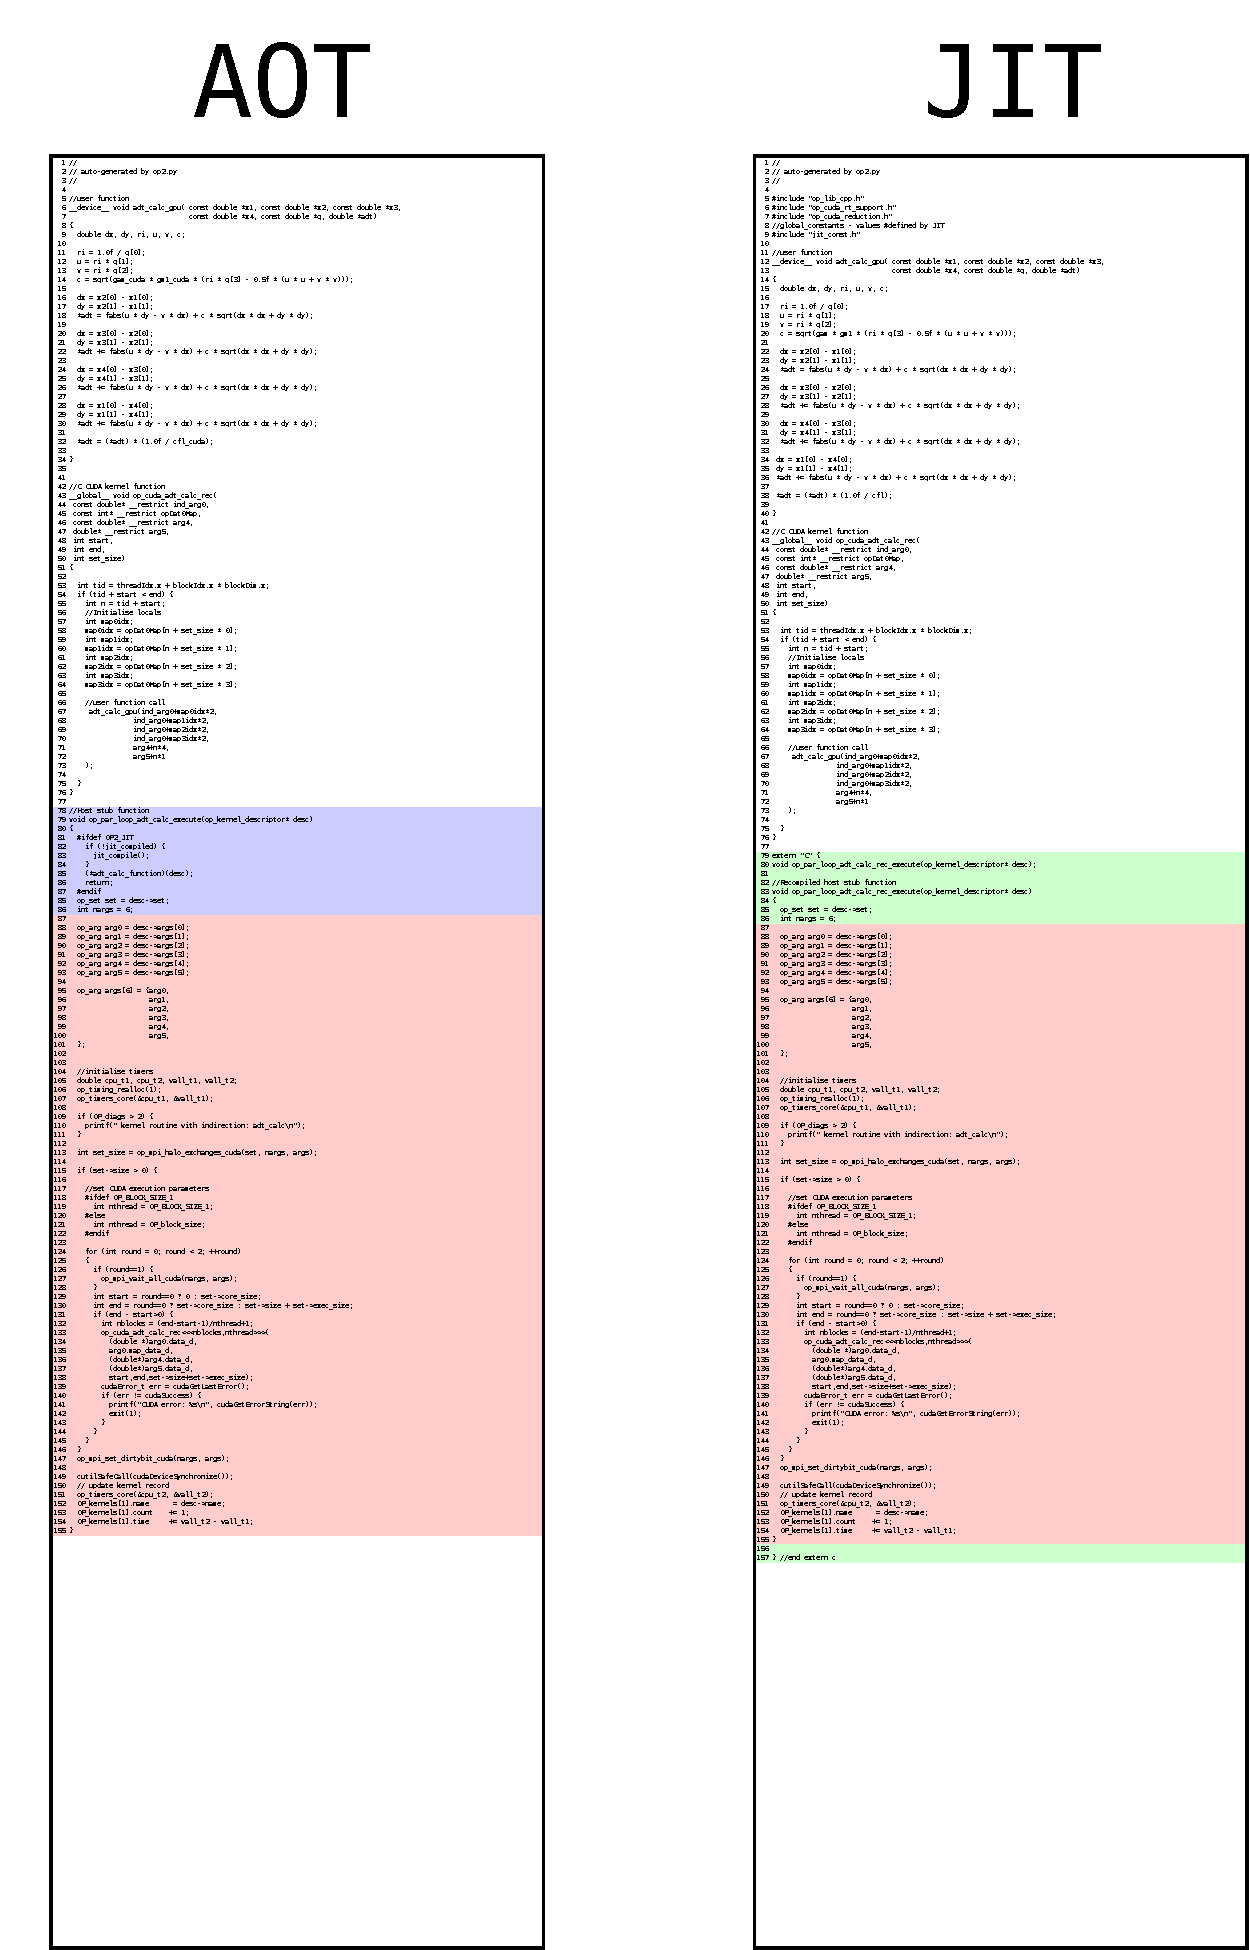
\includegraphics[width=.3\textwidth]{host_function}
\end{wrapfigure}
\minititle{Host Function}
The purpose of the host function is to bridge the gap between the host and the device. It is CPU code, so runs on the host, but contains the CUDA call to the kernel function which will run on the GPU. While the function body is the same for both AOT and JIT: setting up arguments, timers, and block and thread sizes for the CUDA call; the function head differs, as shown in Figure \ref{fig:host_func}.
\vspace{\parskip}

\tinytitle{AOT}
In the Ahead-Of-Time kernel file, the C code generated for the head of the host function is as follows:

\begin{lstlisting}[linewidth = \textwidth, framesep=0pt, language=C, linebackgroundcolor={\ifnum\value{lstnumber}=14\color{red!20} \else \color{blue!20} \fi}]
 //Host stub function
 void op_par_loop_[name]_execute(op_kernel_descriptor* desc)
 {
   #ifdef OP2_JIT
     if (!jit_compiled) {
       jit_compile();
     }
     (*[name]_function)(desc);
     return;
   #endif

   op_set set = desc->set;
   int nargs = 6;
   ... //Identical Section
 }
\end{lstlisting}
\vspace{-1em}
The function name is \verb|op_par_loop_[name]_execute| because a pointer to this function will be queued by the lazy execution system mentioned previously in this Section, so this function actually executes the loop, whenever the lazy execution system should decide it needs to be executed. The decision of when to call the loop is outside the scope of this project, and currently a loop is simply called immediately after it is queued.
\par At the top of the function a decision is made as to whether JIT should be used, based on whether \verb|OP2_JIT| has been defined. This allows JIT to be turned on and off through the used the compiler argument \verb|-DOP2_JIT|. If JIT is enabled, then the compiler is invoked (if it hasn't been already), and the pointer to the newly compiler version of the function is executed instead.
\par
If JIT is not enabled, this code will be ignored by the compiler, so the process will continue into the AOT host function, which causes it to stay whithin the AOT kernel file and never execute any code from the JIT file.

\tinytitle{JIT}
Contrasting this with the code generated for the JIT kernel file:

\begin{lstlisting}[linewidth = \textwidth, framesep=0pt, linebackgroundcolor={\ifnum\value{lstnumber}=9\color{red!20} \else \color{green!20} \fi}]
 extern "C" {
 void op_par_loop_[name]_rec_execute(op_kernel_descriptor* desc);

 //Recompiled host stub function
 void op_par_loop_[name]_rec_execute(op_kernel_descriptor* desc)
 {
   op_set set = desc->set;
   int nargs = 6;
   ... //Identical Section
 }

 } //end extern c
\end{lstlisting}
\vspace{-1em}

Firstly, since this function needs to be linked to the exisiting code as part of a dynamically loaded library, it is placed inside an \verb|extern "C"| scope, to ensure C linkage, and prevent the compiler from "mangling" the name. Following that, the function, which is named\\
\verb|op_par_loop_[name]_rec_execute| ("rec" short for recompiled), will come to reside in the address of the \verb|[name]_function| function pointer.
\par
It will be executed after the run-time compiler has been invoked, as the replacement JIT-compiled host function, and make calls to the kernel and user functions in the same file as iteself, rather than those in the AOT file - allowing the optimisations made to be used.

\minititle{Loop Function}
The last section to be generated in the kernel files is the Loop Function, which is the entry point for the parallel loop:
\codeline{op_par_loop_[name](char* name, op_set set, [args]... )}{}

\begin{wrapfigure}[12]{r}{.33\textwidth}
  \vspace{-3em}
  \centering
  \caption{Loop Function}
  \label{fig:loop_func}
  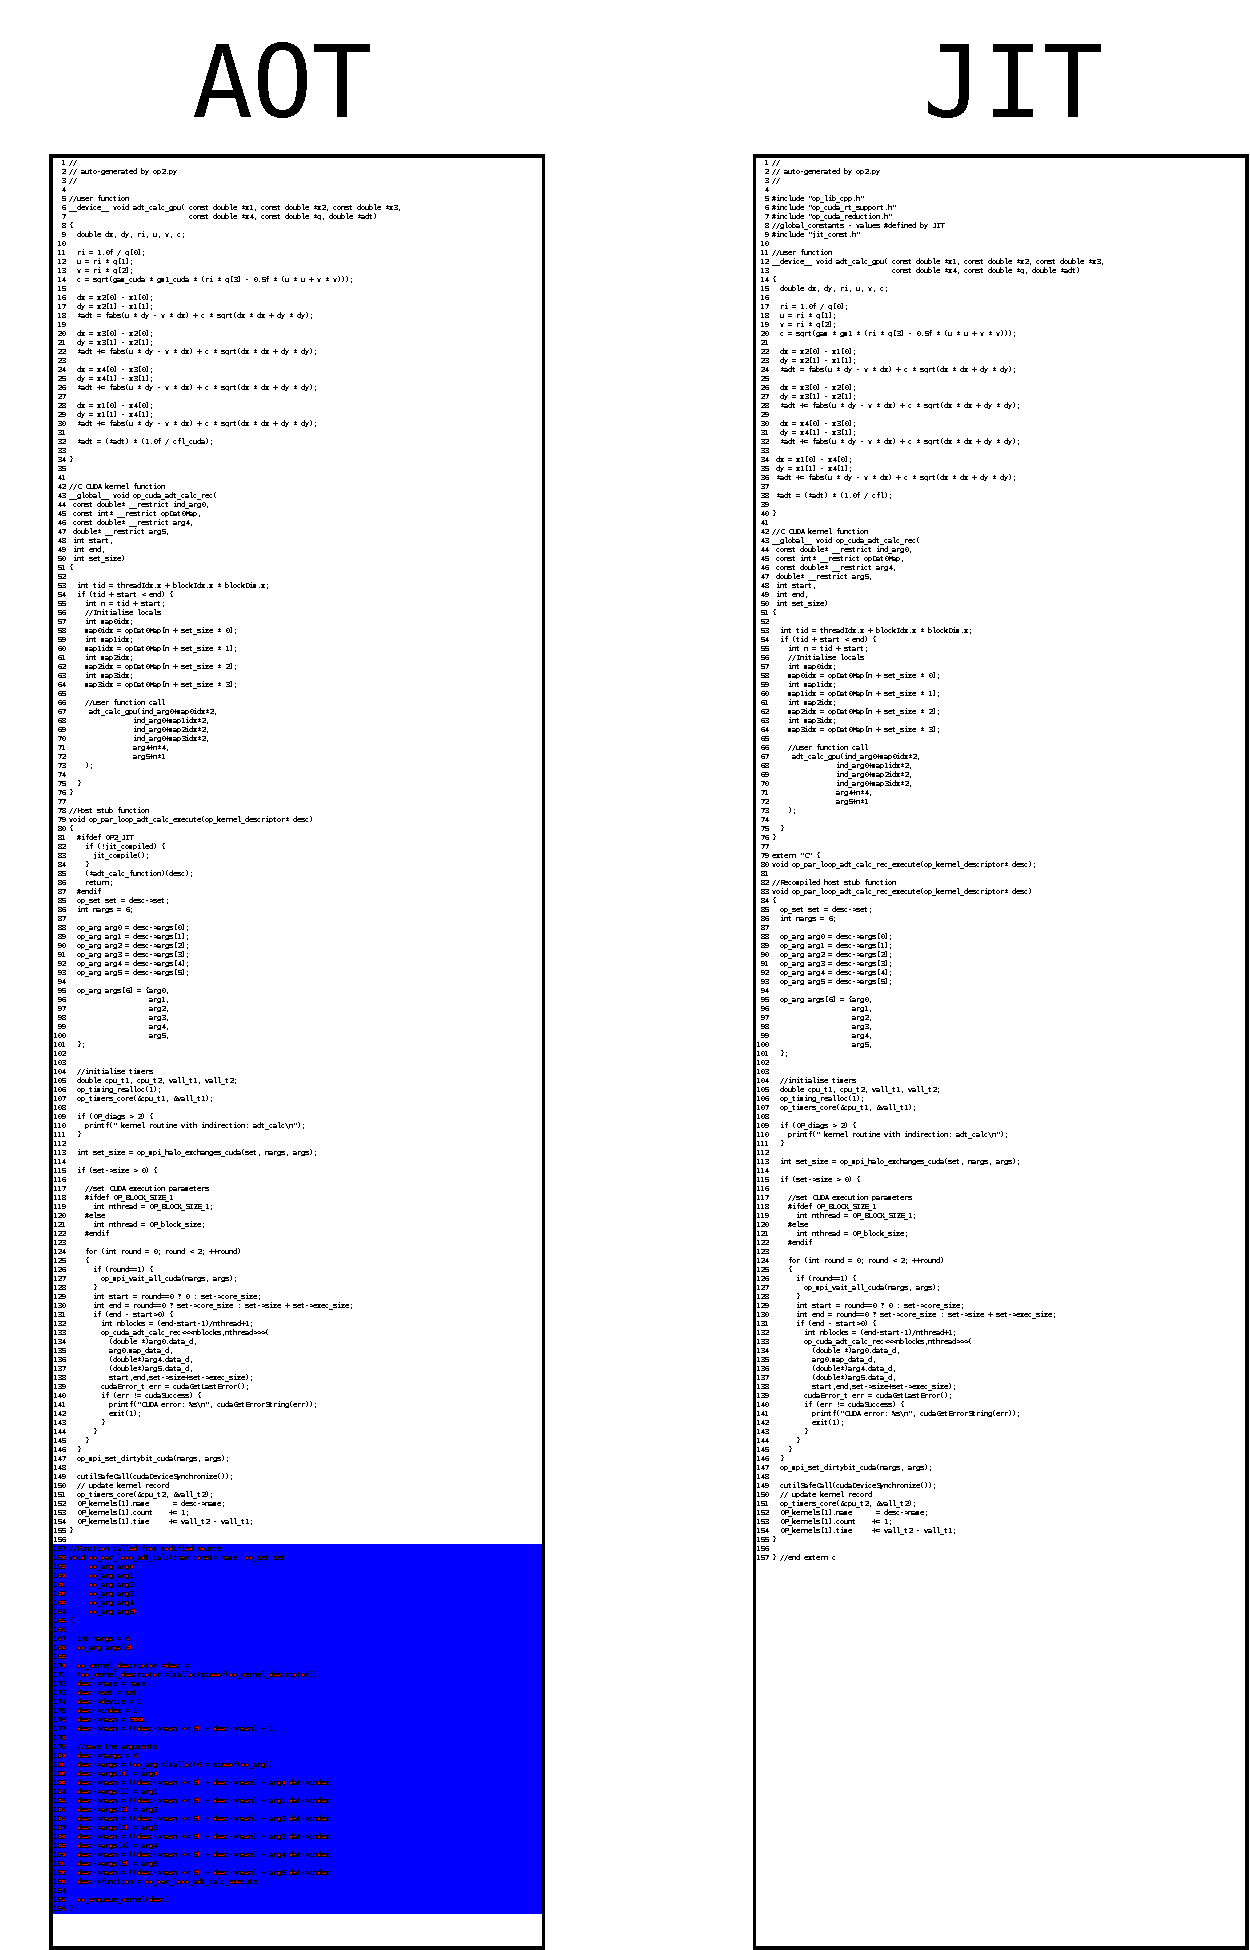
\includegraphics[width=.3\textwidth]{loop_function}
\end{wrapfigure}
The application file will be modified by \verb|op2.py| to contain an declaration for this function marked \verb|extern|, to be linked againt this definition. Only the AOT kernel requires this, as previously mentioned the JIT host function acts as its entry point (Figure \ref{fig:loop_func}).
\\
The purpose of this function is to generate the kernel descriptor, then make a call to:
\codeline{void op_enqueue_kernel(op_kernel_descriptor *desc)}{op2/c/src/core/op\_lazy.cpp [71-89]}

\noindent As previously mentioned, the kernel descriptor and enqueue function were part of the work done to enable lazy execution in OP2, and not created as part of this project.

\vspace{2em}

\begin{wrapfigure}[13]{l}{.4\textwidth}
  \vspace{-2em}
  \centering
  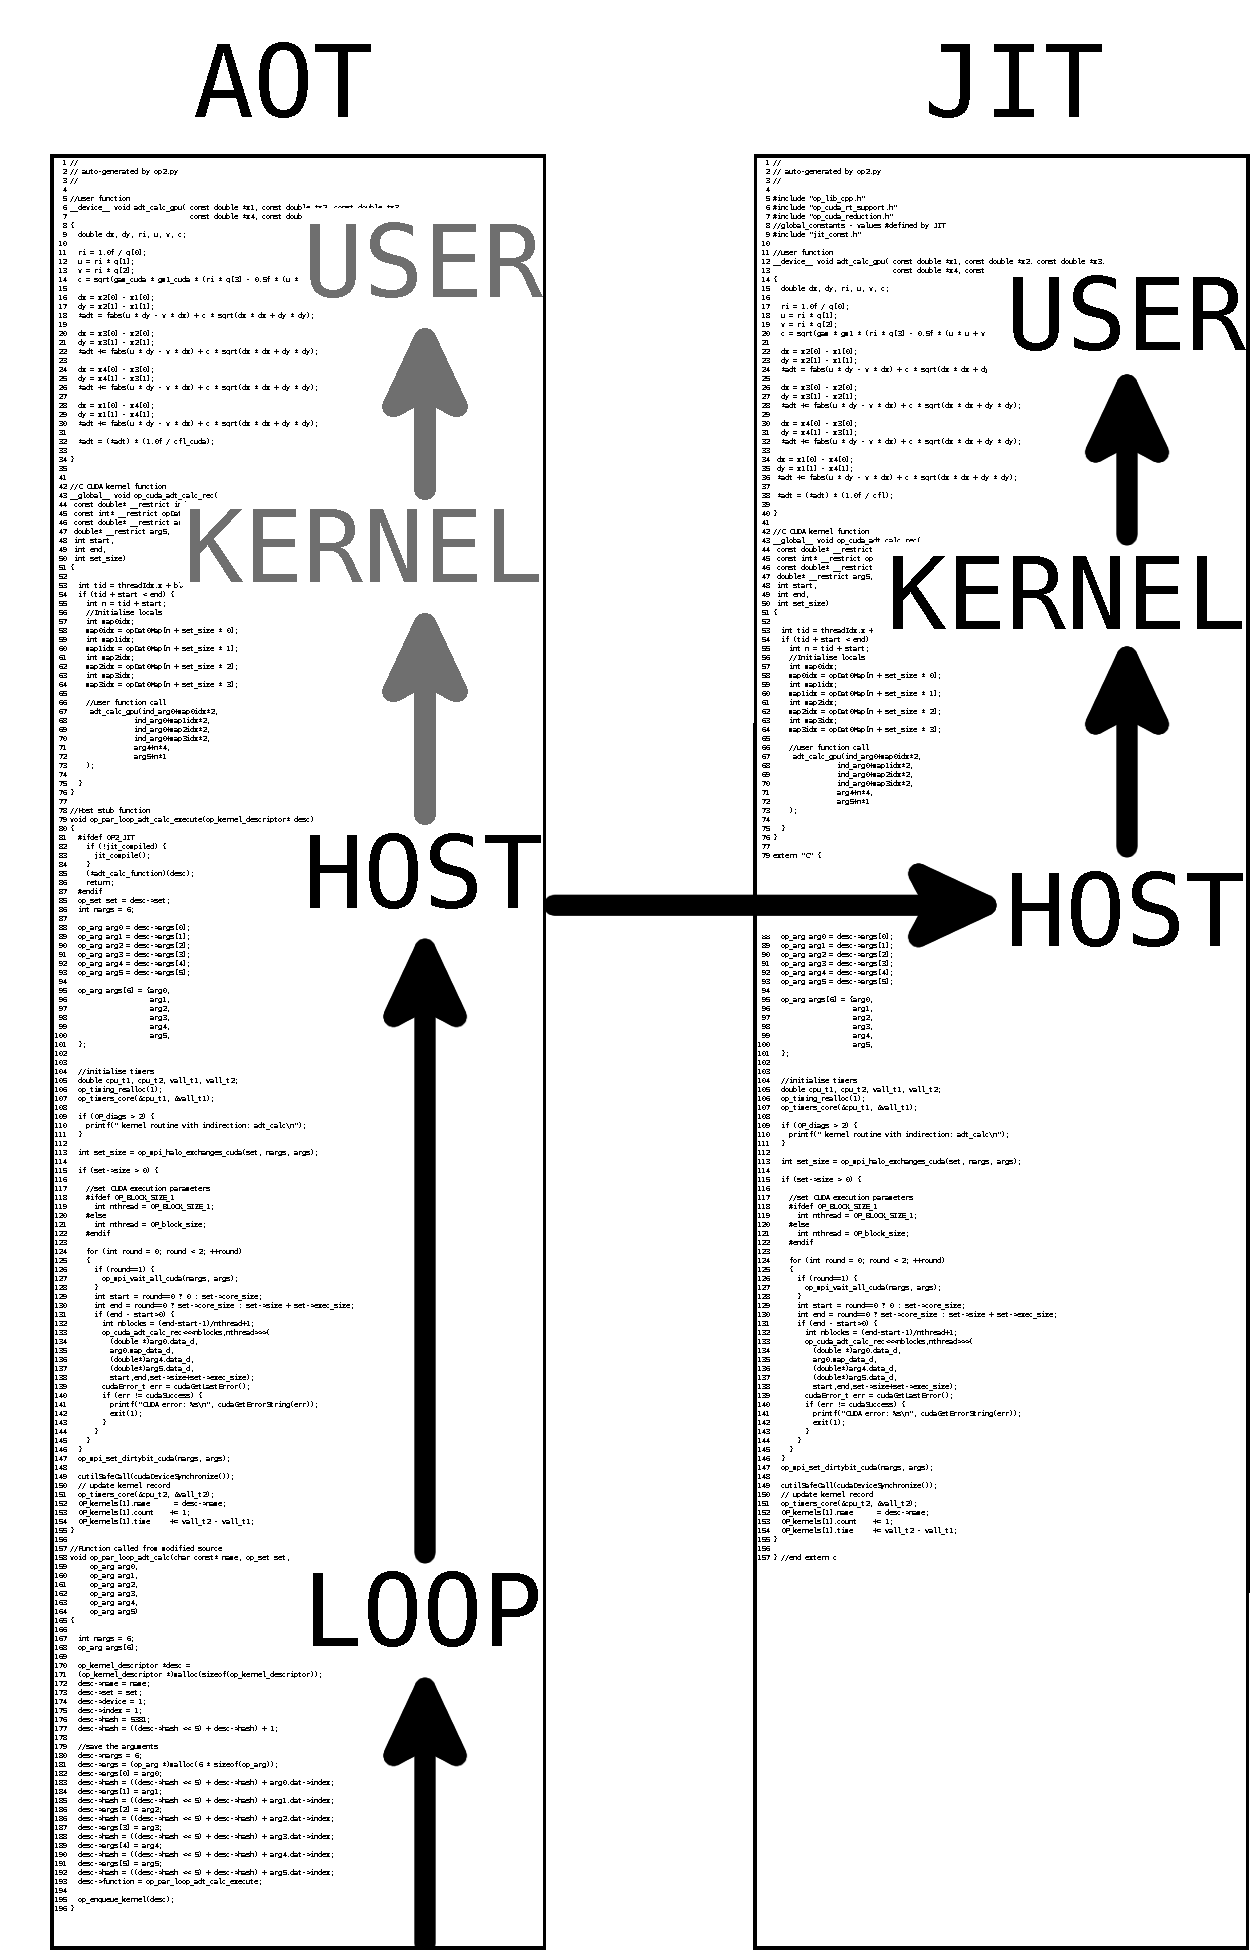
\includegraphics[width=.39\textwidth]{krnl_flow}
  \caption{Kernel Flow}
  \label{fig:krnl_flow}
\end{wrapfigure}

\tinytitle{Summary}
\label{impl_summary}

To recap, the AOT and JIT kernel files are generated for each parallel loop, to be executed when that loop is invoked in the application file. Figure \ref{fig:krnl_flow} has been included to make clear the data flow through the two files: starting in the Loop Function, which calls the AOT Host Function, where either the re-compiled version is invoked, or the original version is used if JIT is not enabled at compile time.

The \verb|jit_compile()| function has not yet been defined, but this will be covered in the next section on the master kernels file.
\clearpage
\subsubsection{Master Kernels File}
\label{sss:mkf}
The Master Kernels File: \verb|cuda/[application]_kernels.cu| is the last file to be generated, once the kernels for each parallel loop have been completed. It ties up most of the remaining loose ends, as it contains shared functions for invoking the run-time compiler, and declaring constants. It also contains \verb|#include| statements for each of the AOT kernel files, so that the application file can be linked against this file only at compile-time, and the linker will be able to find definitions for all the functions declared extern. The Makefile and compile process will be covered further in Section TODO.
\par
At the top, the master kernels file includes the requried OP2 library files. It then defines a CUDA constant for each constant the user has defined, generated using the following python code:
\begin{lstlisting}[backgroundcolor = \color{lightgray!20}, language=Python]
for nc in range (0,len(consts)):
  if consts[nc]['dim']==1:
    # __constant__ [type] [name]_cuda;
    code('__constant__ ' + consts[nc]['type'][1:-1] + ' ' +
          consts[nc]['name'] + '_cuda;')
  else:
    if consts[nc]['dim'] > 0:
      num = str(consts[nc]['dim'])
    else:
      num = 'MAX_CONST_SIZE'

    # __constant__ [type] [name]_cuda[ [dim] ];
    code('__constant__ ' + consts[nc]['type'][1:-1] + ' ' +
          consts[nc]['name'] + '_cuda' + '['+num+'];')
\end{lstlisting}
\vspace{-1em}
\hspace*{\fill}\footnotesize{translator/c/python/jit/op2\_gen\_cuda\_jit.py [974-985]
\\
Following this, the file contains definitions for two functions. The first is \verb|op_decl_const_char|, which will be called from the application file to declare a constant identifier and value; and the second is \verb|jit_compile| which will invoke the run-time compiler, load the generated DLL and create a function pointer for each re-compiled loop.

\minititle{op\_decl\_const\_char}
This function is an OP2 library function which allows users to declare a value that will not change over the course of execution. It has the following signature, defined by the OP2 API\cite[p9]{manual}:
\codeline{void op_decl_const_char(int dim, char const *type, int size,
                                  char *dat, char const *name)}{}
 Two versions of the function are generated, one for AOT and one for JIT. The two functions are wrapped with pre-processor conditionals, so that only one of them will be visible to the compiler. As before, \verb|OP2_JIT| being defined is the test, so the JIT functionality can be enabled or disabled.
\par
The AOT version of the function copies the value passed to it to the corresponding device constant using:
\codeline{cudaMemcpyToSymbol(const void* symbol, const void* src, size_t count)}{}
The copy default direction for this function is from host memory to device memory.
\par
The JIT version instead invokes the internal library function:
\codeline{void op_lazy_const(int dim, char const *type, int typeSize, char *data,
                        char const *name)}{op2/c/src/core/op\_lazy.cpp [100-101]}
Which maintains a de-duplicated list of constants, so that once they all have been declared the header file defining their values can be generated. As can be seen in the generated C code below, constants containing more than one value are declared as single values due to the issues with \verb|extern __constant__| values described in Section \ref{ss:krnl_files} (2. User Function).
\begin{lstlisting}[linewidth = \textwidth, framesep=0pt]
void op_decl_const_char(int dim, char const *type,
                        int size, char *dat,
                        char const *name)
{
  if (dim == 1) {
    op_lazy_const(dim, type, size, dat, name);
  }
  else {
    for (int d = 0; d < dim; ++d)
    {
      char name2[32];
      sprintf(name2, "op_const_%s_%d\0", name, d);
      op_lazy_const(1, type, size, dat+(d*size), name2);
    }
  }
}
\end{lstlisting}
\vspace{-1em}
\hspace*{\fill}\footnotesize{generated by translator/c/python/jit/op2\_gen\_cuda\_jit.py [1028-1046]}

\minititle{jit\_compile}
The other function generated is the \verb|jit_compile| function, which is responsible for the actual recompilation of the JIT kernels, and making their functions available to the binary. It also uses the same timing library functions which gather data on the time spent in each parallel loop to determine how long the binary spends re-compiling, as this is important for performance measuring later.
\par
The compiler arguments, library paths, and other required parameters are in this implementation handled by a make file which would need to be generated by the user. The contents of the makefile will be covered in the next section.
\par
As can be seen below, the executable makes a system call to initiate a make command, and stores the result in a log file. If the compilation fails, an error message is printed, and the program exits early.
\begin{lstlisting}[linewidth = \textwidth, framesep=0pt]
if (op_is_root()) {
  if (system("make -j [application]_cuda_rec &> jit_compile.log"))
  {
    // 0 indicated success
    printf("Error: JIT compile failed. \n
            - see jit_compile.log for details\n");
    exit(1);
  }
}
\end{lstlisting}
\vspace{-1em}
\hspace*{\fill}\footnotesize{generated by translator/c/python/jit/op2\_gen\_cuda\_jit.py [1071-1077]}

It is expected that the make file will generate a shared object file named \verb|cuda/airfoil_kernel_rec.so|. If this file does not exist the binary exits with an error, otherwise the recompiled function for each parallel loop is dynamically loaded using:
\codeline{void *dlsym(void *restrict handle, const char *restrict name);}{dlfcn.h}
The function \verb|op_par_loop_[name]_rec_execute| loaded, with the address stored in a void pointer with identifer \verb|[name]_function|. We have seen this pointer before in Section \ref{ss:krnl_files} (4. Host Function).
\par
Once this has been done for all loops, the wall clock time since the start of the \verb|jit_compile| function is printed to the terminal.

\subsection{Makefile}
This implementation relies on GNU Make\cite{make} to determine which compiler should be used, which parameters should be passed, and other options. There are a number of libraries required to build an OP2 binary, as covered in Appendix \ref{app:getStart}, so only the recompilation target will be discussed here.
\par
The binary expects there to be a Makefile in the directory it executes in, with a target: \verb|[application]_cuda_rec| in order to work correctly. This is the target which will be compiled at run-time. As mentioned in the previous section, the result of making this target needs to be a a shared object file named \verb|cuda/airfoil_kernel_rec.so|, which contains the recompiled loop functions.
\par
The library object is produced by compiling each of the kernels individually, using the NVidia compiler \verb|nvcc| from the NVidia CUDA Toolkit\cite{nvcc,toolkit} as the code contains CUDA, then linking them into a single object. It is necessary that the compiler flags include \verb|--compiler-options -fPIC|. This passes a list of arguments to the underlying compiler, since nvcc only handles the CUDA code, and passes all host code compilation on to a C compiler. The argument to be passed down is \verb|-fPIC|, to generate Position Independant Code, to allow the library function to execute correctly, regardless of the address at which it is loaded in memory.
\subsubsection{Optional Functionality}
By default, the JIT compilation functionality is enabled in the Makefile by setting the value of \verb|$JIT| to \verb|TRUE|. However, if the variable is set to anything else in the parameters of the make command, JIT will be disabled in the resulting executable. This is done with the following lines:
\begin{lstlisting}[linewidth = \textwidth, framesep=0pt]
ifeq ($(JIT), TRUE)
	CCFLAGS    := $(CCFLAGS) -DOP2_JIT
	NVCCFLAGS  := $(NVCCFLAGS) -DOP2_JIT
	SUFFIX     := _jit
endif
\end{lstlisting}
Which adds a parameter to the C and CUDA compilers to define \verb|OP2_JIT| for the preprocessor, and appends "\_jit" to the name of the executable generated.
\par
The target \verb|cuda/airfoil_kernels_cu.o| is also declared PHONY, so that it is always recompiled even if the file already exists, otherwise this make flag would not function correctly, and a JIT enabled version of this file may be used when the user intended to recompile it with JIT disabled.
